\chapter{Resultados}
\label{chap:resultados}
A fase de desenvolvimento do robô Doogie culminou em 4 resultados principais: Protótipo, ambiente de simulação, labirinto para testes e competição e a estrutura de software da plataforma móvel. Os tópicos posteriores irão detalhar cada um desses resultados. 

%--------- NEW SECTION ----------------------
\section{Protótipo}
\label{sec:resultado_prototipo}

\begin{figure}[H]
	\centering
	\caption{Componentes da placa superior do Doogie Mouse}
	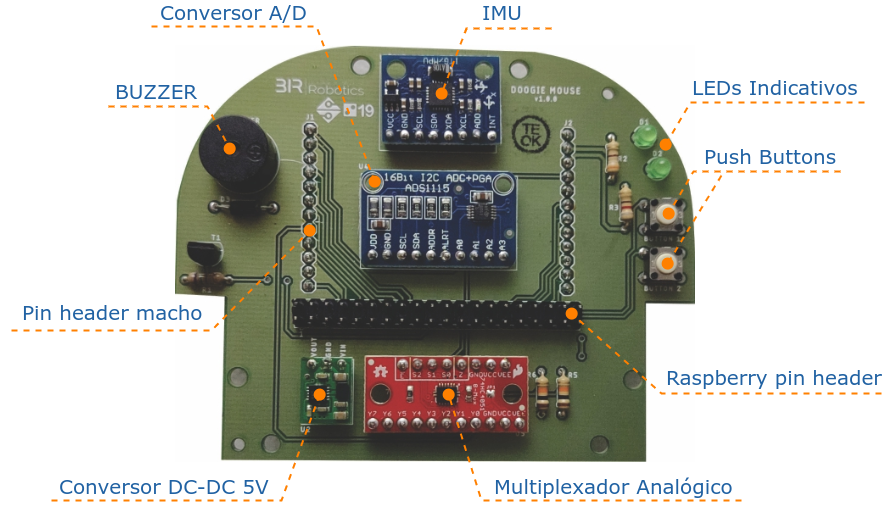
\includegraphics[width=1\textwidth]
	{Figures/top_board_elementos.png}
	\label{fig:top_board_elementos}
	\source{Própria Autoria}
\end{figure}

\begin{figure}[H]
	\centering
	\caption{Componentes da placa inferior do Doogie Mouse}
	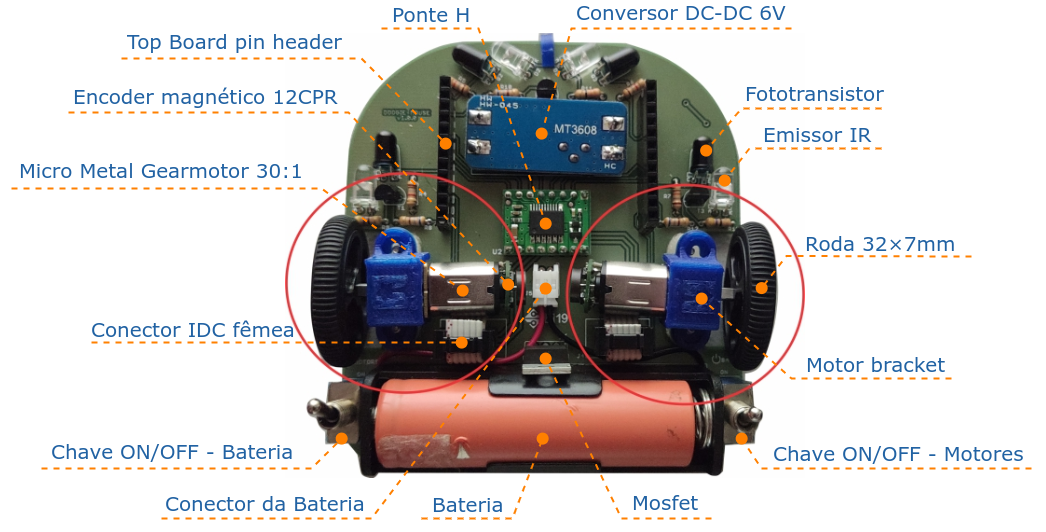
\includegraphics[width=1\textwidth]
	{Figures/bottom_board_elementos.png}
	\label{fig:bottom_board_elementos}
	\source{Própria Autoria}
\end{figure}

\begin{figure}[H]
	\centering
	\caption{Protótipos do Doogie Mouse confeccionados}
	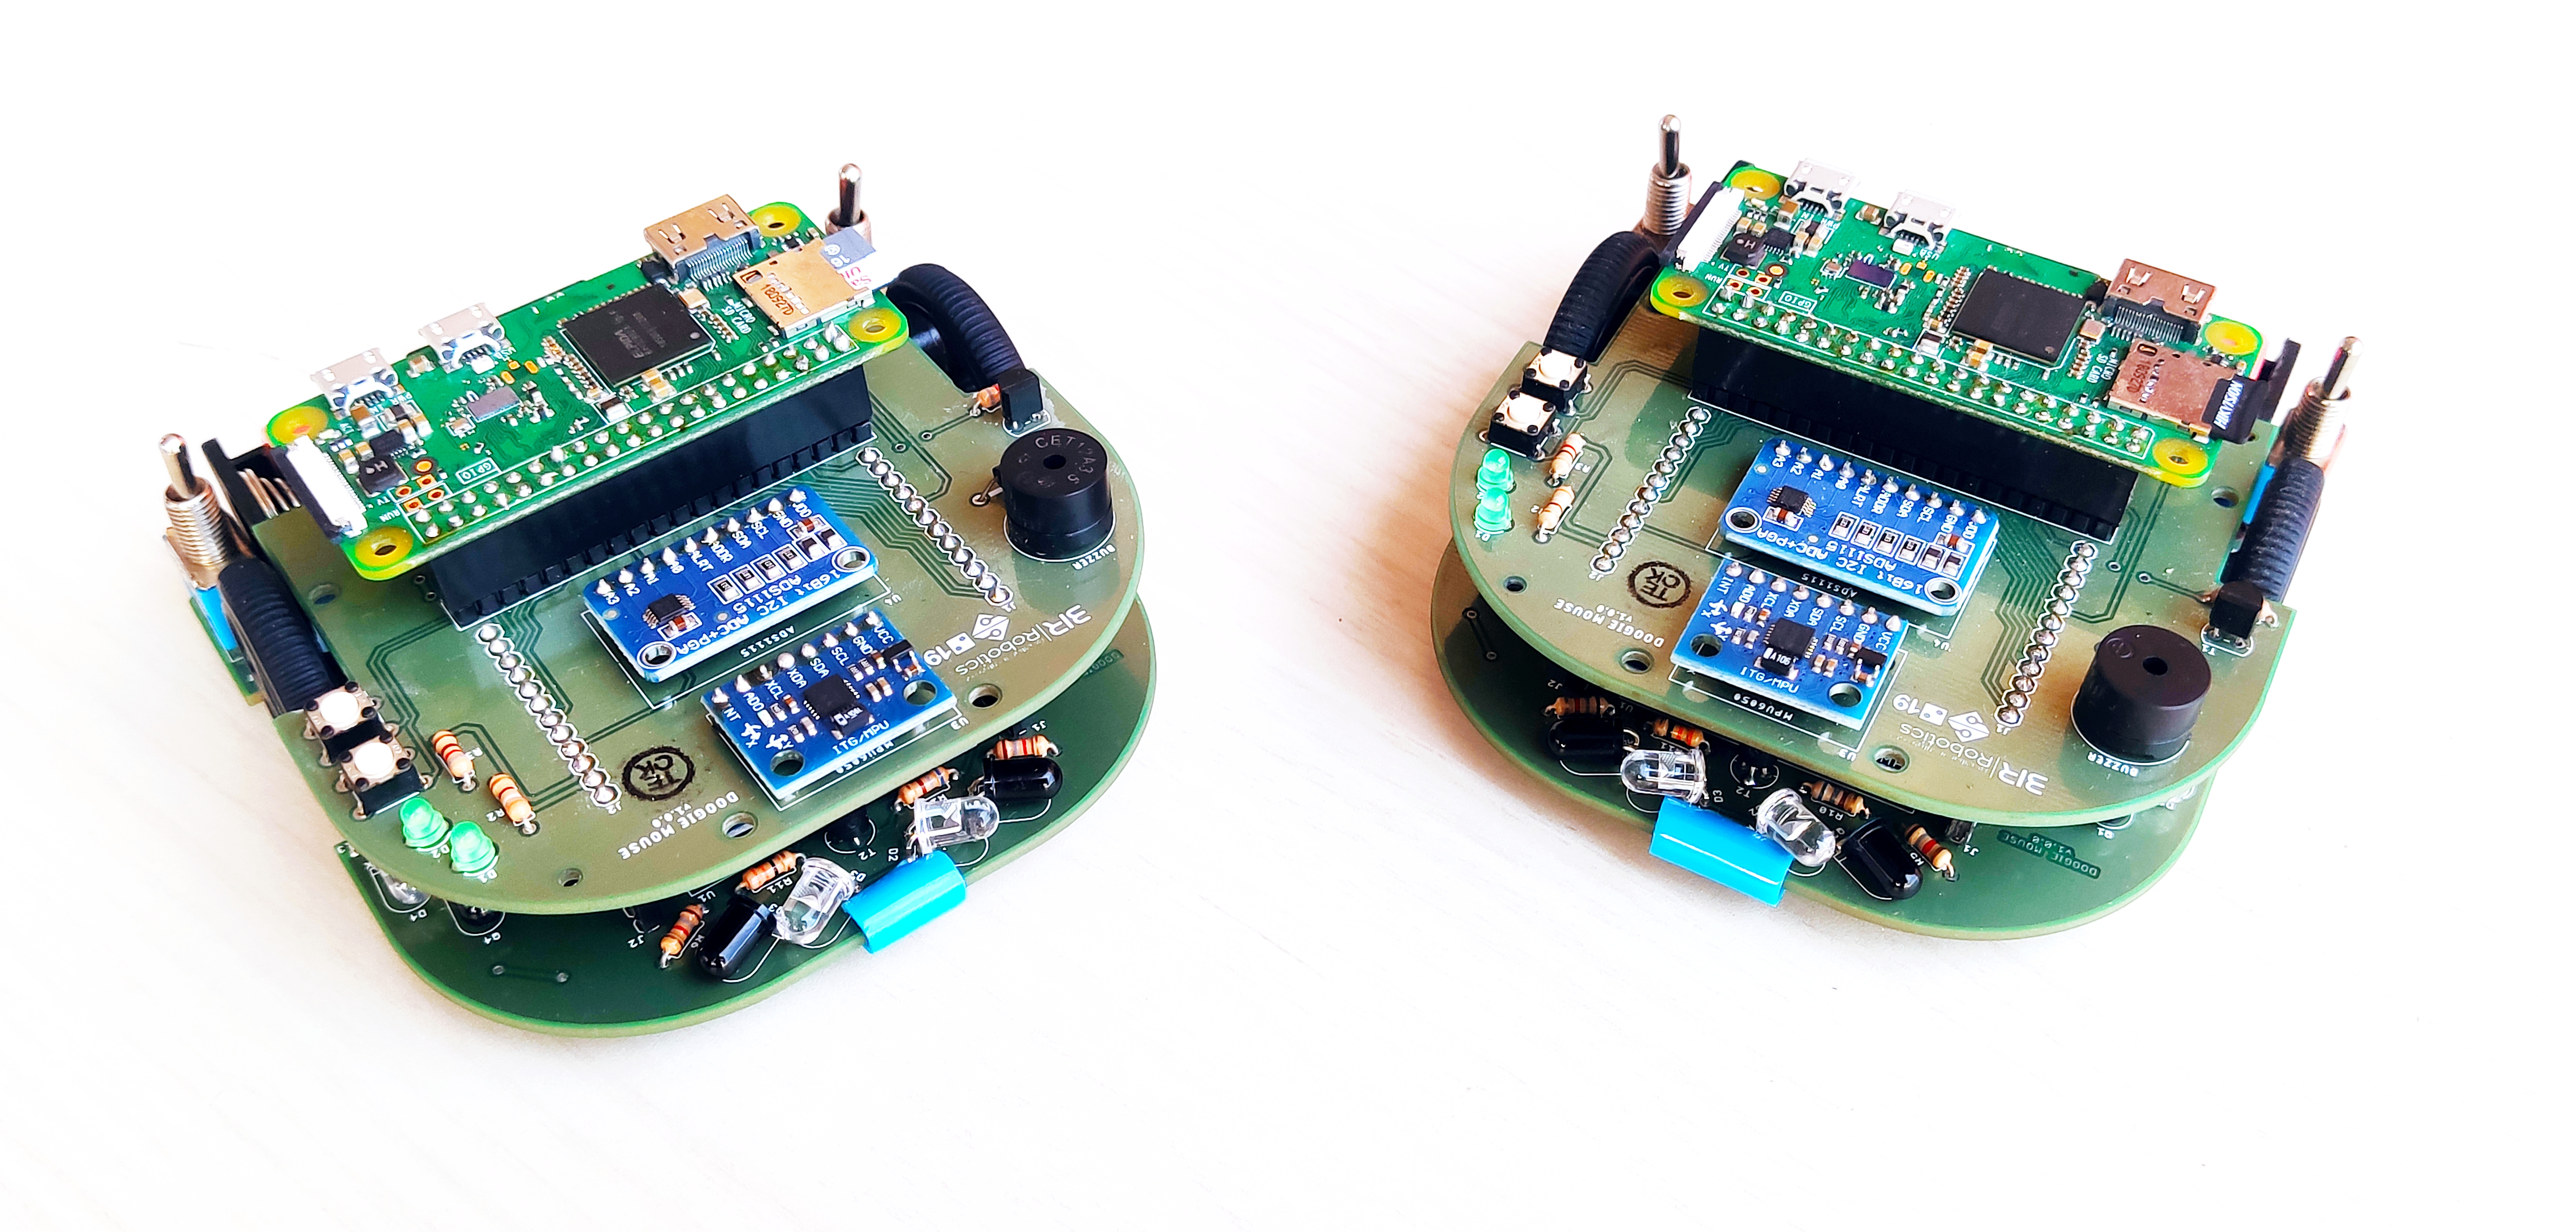
\includegraphics[width=1\textwidth]
	{Figures/doogie_mouse_prototipos}
	\label{fig:prototipos}
	\source{Própria Autoria}
\end{figure}

\section{Ambiente de simulação}
\label{sec:resultado_ambiente_de_simulacao}
hhajshfdsahf

%--------- NEW SECTION ----------------------
\section{Labirinto}
\label{sec:resultado_labirinto}
asdfadsfsdfs

%--------- NEW SECTION ----------------------
\section{Estrutura de Software}
\label{sec:resultado_estrutura_de_software}
Para contemplar o objetivo do projeto, que é ser uma plataforma para aprendizagem de robótica móvel e inteligência artificial, optou-se pelo uso do \textit{framework} \gls*{ros} devido a sua capacidade de abstração de hardware e de reuso de software como já mencionado em \ref{sec:robotic_frameworks}






